\chapter{Finite State-Machines}
\label{cha:logic}
    \tikzstyle{state} = [rectangle, draw=none, rounded corners=1mm, fill=YellowGreen,
                    text centered, anchor=north, text=white, minimum width=2.5cm, minimum height=1cm, node distance=3cm, align=center]
    \tikzstyle{condition} = [diamond, draw=none, fill=red!80,
                    text centered, anchor=north, text=white, minimum height=1cm, node distance=3cm, align=center]
    \tikzstyle{choice}=[font=\scriptsize]

    In projects related to the LinkQuad quadrotor, generic state-machine
    frameworks have been developed and researched\citep{Merz06,Wzorek11}.
    On the LinkQuad, for the purpose of this thesis, a stripped down state-machine engine
    was implemented in the \textit{CRAP} framework presented in Appendix \ref{app:crap}.

    The state machine is responsible for transitioning between the
    states - action modes - predefined in an action sequence, ultimately
    providing reference signals for the controller.

    \section{Implemented Modes}
        In this Section, four basic modes are presented which were implemented
        in the timeframe of this thesis.

        \subsection{Hovering}
            In the hover mode, the position of the quadrotor is noted at
            the time of the activation, and three independent PID-controllers
            are initialized to generate reference signals to the main controller,
            working to keep the quadrotor at the place where it was first initialized.
            \begin{figure}[h]
                \noindent\makebox[\textwidth]{%
                    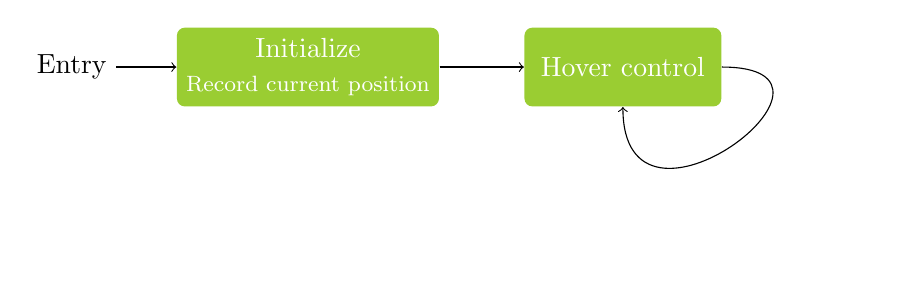
\begin{tikzpicture}[auto]
                        \node (entry) {Entry};
                        \node [state, right of=entry,text centered, align=center, node distance=3cm] (init) {Initialize \\ \footnotesize{Record current position}};
                        \node [state, right of=init, node distance=4cm] (hover) {Hover control};
                        \path[->]
                            (entry.east) edge (init.west)
                            (init.east) edge (hover.west)
                            (hover.east) edge [loop below, out=0, in=-90, distance=2cm] (hover.south);
                    \end{tikzpicture}
                }
                \caption{Hovering scheme.}
                \label{fig:logic:hoverscheme}
            \end{figure}

        \subsection{PTAM initialization}
            Entering this mode starts an automated initialization process
            to set up the initial PTAM coordinate system. Commands are sent
            to the PTAM module to initialize tracking, after which
            the quadrotor should be moved sideways for the
            stereo initialization performed by the PTAM library.
            %~ while the control reference is adjusted to move the quadrotor slowly sideways for the
            %~ stereo initialization performed by the PTAM library.

            %~ \textbf{Insert tikz here}

        \subsection{Free Flight}
            In the free flight mode, the control reference is forwarded
            from the joystick reference provided over the serial interface
            from the ground station.

            \begin{figure}[h]
                \noindent\makebox[\textwidth]{%
                    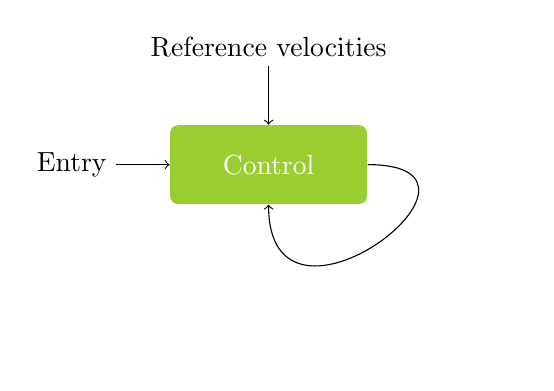
\begin{tikzpicture}[auto]
                        \node (entry) {Entry};
                        \node [state, right of=entry, node distance=2.5cm] (control) {Control};
                        \node [above of=control, node distance=1.5cm] (reference) {Reference velocities};
                        \path[->]
                            (entry.east) edge (control.west)
                            (reference.south) edge (control.north)
                            (control.east) edge [loop below, out=0, in=-90, distance=2cm] (control.south);
                    \end{tikzpicture}
                }
                \caption{Freeflight scheme}
                \label{fig:logic:freeflightscheme}
            \end{figure}

        \subsection{Landing}
            \label{ssec:logic:landing}
            There have been several studies of autonomous quadrotor landing,
            in e.g.\citep{mellinger10perching,brockers:803111}.
            \citep{brockers:803111} implements a landing scheme closely related to
            that which is proposed in this thesis.
            The algorithm used can be summarized in the following steps:
            \begin{itemize}
                \item Detection,
                \item Refinement,
                \item Descent,
                \item Landig detection.
            \end{itemize}

            In the detection phase, the environment is searched for a suitable
            landing place. Landing is then performed on an elevated surface which is detected using video processing.
            After the landing area has been located, the position of the
            landing site - relative to the quadrotor - is filtered to increase the
            certainty of the positioning.

            \begin{figure}[h]
                \noindent\makebox[\textwidth]{%
                    \begin{tikzpicture}[auto]
                        \node (entry) {Entry};
                        \node [state, right of=entry] (halt) {Halt to hover\\ \footnotesize{Set $V_{ref}=0$}};
                        \node [condition,right of=halt] (halted) {$|V| < \epsilon$};
                        \node [state, below of=halt, node distance=2cm] (descend) {Descend \\ \footnotesize{Set $V_{ref,z} > 0$}};
                        \node [condition,right of=descend] (landed) {Landed};
                        \node [state, below of=descend, node distance=2cm] (spindown) {Spin down};
                        \path[->]
                            (entry.east) edge (halt.west)
                            (halt.east) edge (halted.west)
                            (halted.east) edge [loop right,distance=2cm, in=45,out=-45] node [choice] {No} (halted.east)
                            (halted) edge [loop right,in=90,out=-135] node [choice,yshift=0.2cm] {Yes} (descend.north)
                            (descend.east) edge (landed.west)
                            (landed.east) edge [loop right,distance=2cm, in=45,out=-45] node [choice] {No} (landed.east)
                            (landed) edge [loop right,in=90,out=-135] node [choice,yshift=0.2cm] {Yes} (spindown.north)
                    %       (control.east) edge [loop below, out=0, in=-90, distance=2cm] (control.south)
                        ;
                    \end{tikzpicture}
                }
                \caption{Landing scheme.}
                \label{fig:logic:landingscheme}
            \end{figure}

            While the filtered position converges, the quadrotor is moved to
            a position above the landing site as preparation for the descention phase,
            where the quadrotor lowers until landing has been detected,
            using the camera feedback and other sensors to stabilize the descent.

            \subsubsection{Landing Detection}
                Since we recognize that our estimated position - with origin at our starting point -
                is not nescessarily consistent with the Height Over Ground (HOG)
                at the landing site, it is nescessary to choose a more robust
                method to detect the completion of the landing procedure than simply halting at zero height.
                The approach is to use the measurements to determine when movement
                has stopped; that is, when the quadrotor has reached ground.
                Detection theory, as discussed in e.g. \citep{Tornqvist08,nyberg11diagnosis},
                provides several tools for detecting the non-linear event that
                the quadrotor can descend no further.

                In the physical model presented in Chapter \ref{cha:observer},
                two terms is of specific interest for the detection.
                The first - and the obvious - is the velocity in the gravity-aligned z-axis.
                When sensor measurements pull this term towards zero,
                this is a first indication that the quadrotor has stopped.
                When the sensor measurements indicate a halt, the
                observer - oblivious to the forces imposed by the
                ground contact - will explain the lack of movement by a drastic increase in
                the estimated wind acting in the z-direction.
                This observer state - the second of interest - is easily monitored
                and could e.g. be filtered using the Cumulative Sum (CUSUM) algorithm to
                increase detection confidence, or simply thresholded to detect landing.
